\documentclass{scrartcl}
\usepackage{mathtools}
\usepackage{tikz}
\usetikzlibrary{trees,positioning}

\begin{document}
\begin{figure}
\centering
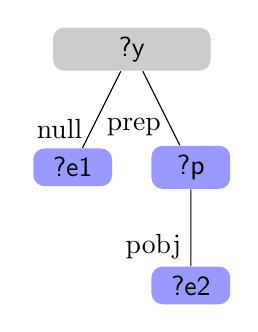
\begin{tikzpicture}
\node[fill = gray!40, shape = rectangle, rounded corners, minimum width = 2cm, font = \sffamily] (0) {?y}
child {node[fill = blue!40, shape = rectangle, rounded corners, minimum width = 1cm, font = \sffamily]  (1) {?e1}
}
child {node[fill = blue!40, shape = rectangle, rounded corners, minimum width = 1cm, font = \sffamily]  (2) {?p}
child {node[fill = blue!40, shape = rectangle, rounded corners, minimum width = 1cm, font = \sffamily] (3) {?e2}
}
};
\begin{scope}[nodes = {draw = none}]
\path (1)     -- (0) node [near start, left]  {\text{null}};
\path (2)     -- (0) node [near start, left]  {\text{prep}};
\path (3)     -- (2) node [near start, left]  {\text{pobj}};
\draw[densely dashed, rounded corners, thin];
\end{scope} 
\end{tikzpicture}
\caption{Visualisation for SPARQLPattern\_EN\_1}
\label{fig:SPARQLPatternEN1}
\end{figure}


\begin{figure}
\centering
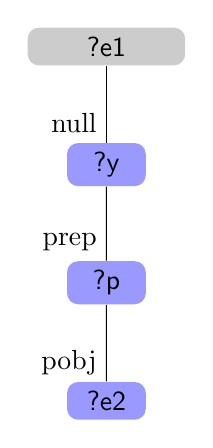
\begin{tikzpicture}
\node[fill = gray!40, shape = rectangle, rounded corners, minimum width = 2cm, font = \sffamily] (3) {?e1}
child {node[fill = blue!40, shape = rectangle, rounded corners, minimum width = 1cm, font = \sffamily]  (4) {?y}
child {node[fill = blue!40, shape = rectangle, rounded corners, minimum width = 1cm, font = \sffamily] (5) {?p}
child {node[fill = blue!40, shape = rectangle, rounded corners, minimum width = 1cm, font = \sffamily] (6) {?e2}
}
}};
\begin{scope}[nodes = {draw = none}]
\path (4)     -- (3) node [near start, left]  {\text{null}};
\path (5)     -- (4) node [near start, left]  {\text{prep}};
\path (6)     -- (5) node [near start, left]  {\text{pobj}};
\draw[densely dashed, rounded corners, thin];
\end{scope} 
\end{tikzpicture}
\caption{Visualisation for SPARQLPattern\_EN\_2}
\label{fig:SPARQLPatternEN2}
\end{figure}


\begin{figure}
\centering
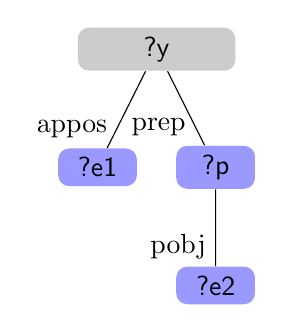
\begin{tikzpicture}
\node[fill = gray!40, shape = rectangle, rounded corners, minimum width = 2cm, font = \sffamily] (6) {?y}
child {node[fill = blue!40, shape = rectangle, rounded corners, minimum width = 1cm, font = \sffamily]  (7) {?e1}
}
child {node[fill = blue!40, shape = rectangle, rounded corners, minimum width = 1cm, font = \sffamily]  (8) {?p}
child {node[fill = blue!40, shape = rectangle, rounded corners, minimum width = 1cm, font = \sffamily] (9) {?e2}
}
};
\begin{scope}[nodes = {draw = none}]
\path (7)     -- (6) node [near start, left]  {\text{appos}};
\path (8)     -- (6) node [near start, left]  {\text{prep}};
\path (9)     -- (8) node [near start, left]  {\text{pobj}};
\draw[densely dashed, rounded corners, thin];
\end{scope} 
\end{tikzpicture}
\caption{Visualisation for SPARQLPattern\_EN\_3}
\label{fig:SPARQLPatternEN3}
\end{figure}


\begin{figure}
\centering
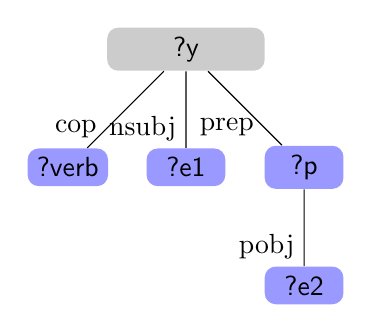
\begin{tikzpicture}
\node[fill = gray!40, shape = rectangle, rounded corners, minimum width = 2cm, font = \sffamily] (9) {?y}
child {node[fill = blue!40, shape = rectangle, rounded corners, minimum width = 1cm, font = \sffamily]  (10) {?verb}
}
child {node[fill = blue!40, shape = rectangle, rounded corners, minimum width = 1cm, font = \sffamily]  (11) {?e1}
}
child {node[fill = blue!40, shape = rectangle, rounded corners, minimum width = 1cm, font = \sffamily]  (12) {?p}
child {node[fill = blue!40, shape = rectangle, rounded corners, minimum width = 1cm, font = \sffamily] (13) {?e2}
}
};
\begin{scope}[nodes = {draw = none}]
\path (10)     -- (9) node [near start, left]  {\text{cop}};
\path (11)     -- (9) node [near start, left]  {\text{nsubj}};
\path (12)     -- (9) node [near start, left]  {\text{prep}};
\path (13)     -- (12) node [near start, left]  {\text{pobj}};
\draw[densely dashed, rounded corners, thin];
\end{scope} 
\end{tikzpicture}
\caption{Visualisation for SPARQLPattern\_EN\_4}
\label{fig:SPARQLPatternEN4}
\end{figure}


\begin{figure}
\centering
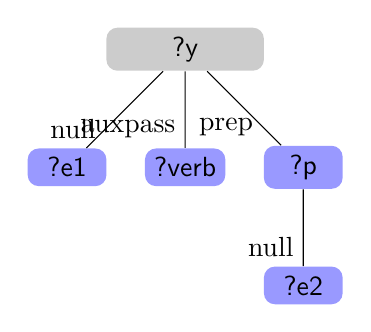
\begin{tikzpicture}
\node[fill = gray!40, shape = rectangle, rounded corners, minimum width = 2cm, font = \sffamily] (13) {?y}
child {node[fill = blue!40, shape = rectangle, rounded corners, minimum width = 1cm, font = \sffamily]  (14) {?e1}
}
child {node[fill = blue!40, shape = rectangle, rounded corners, minimum width = 1cm, font = \sffamily]  (15) {?verb}
}
child {node[fill = blue!40, shape = rectangle, rounded corners, minimum width = 1cm, font = \sffamily]  (16) {?p}
child {node[fill = blue!40, shape = rectangle, rounded corners, minimum width = 1cm, font = \sffamily] (17) {?e2}
}
};
\begin{scope}[nodes = {draw = none}]
\path (14)     -- (13) node [near start, left]  {\text{null}};
\path (15)     -- (13) node [near start, left]  {\text{auxpass}};
\path (16)     -- (13) node [near start, left]  {\text{prep}};
\path (17)     -- (16) node [near start, left]  {\text{null}};
\draw[densely dashed, rounded corners, thin];
\end{scope} 
\end{tikzpicture}
\caption{Visualisation for SPARQLPattern\_EN\_5}
\label{fig:SPARQLPatternEN5}
\end{figure}


\begin{figure}
\centering
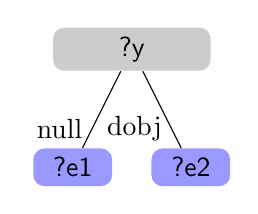
\begin{tikzpicture}
\node[fill = gray!40, shape = rectangle, rounded corners, minimum width = 2cm, font = \sffamily] (17) {?y}
child {node[fill = blue!40, shape = rectangle, rounded corners, minimum width = 1cm, font = \sffamily]  (18) {?e1}
}
child {node[fill = blue!40, shape = rectangle, rounded corners, minimum width = 1cm, font = \sffamily]  (19) {?e2}
}
;
\begin{scope}[nodes = {draw = none}]
\path (18)     -- (17) node [near start, left]  {\text{null}};
\path (19)     -- (17) node [near start, left]  {\text{dobj}};
\draw[densely dashed, rounded corners, thin];
\end{scope} 
\end{tikzpicture}
\caption{Visualisation for SPARQLPattern\_EN\_6}
\label{fig:SPARQLPatternEN6}
\end{figure}


\begin{figure}
\centering
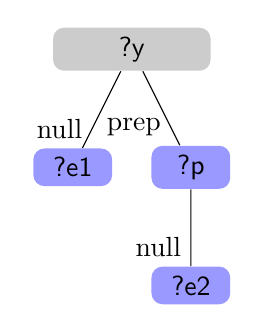
\begin{tikzpicture}
\node[fill = gray!40, shape = rectangle, rounded corners, minimum width = 2cm, font = \sffamily] (19) {?y}
child {node[fill = blue!40, shape = rectangle, rounded corners, minimum width = 1cm, font = \sffamily]  (20) {?e1}
}
child {node[fill = blue!40, shape = rectangle, rounded corners, minimum width = 1cm, font = \sffamily]  (21) {?p}
child {node[fill = blue!40, shape = rectangle, rounded corners, minimum width = 1cm, font = \sffamily] (22) {?e2}
}
};
\begin{scope}[nodes = {draw = none}]
\path (20)     -- (19) node [near start, left]  {\text{null}};
\path (21)     -- (19) node [near start, left]  {\text{prep}};
\path (22)     -- (21) node [near start, left]  {\text{null}};
\draw[densely dashed, rounded corners, thin];
\end{scope} 
\end{tikzpicture}
\caption{Visualisation for SPARQLPattern\_EN\_7}
\label{fig:SPARQLPatternEN7}
\end{figure}


\begin{figure}
\centering
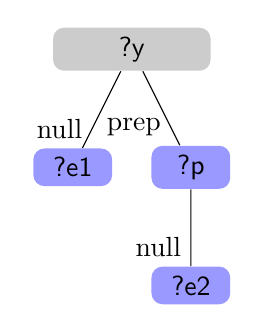
\begin{tikzpicture}
\node[fill = gray!40, shape = rectangle, rounded corners, minimum width = 2cm, font = \sffamily] (22) {?y}
child {node[fill = blue!40, shape = rectangle, rounded corners, minimum width = 1cm, font = \sffamily]  (23) {?e1}
}
child {node[fill = blue!40, shape = rectangle, rounded corners, minimum width = 1cm, font = \sffamily]  (24) {?p}
child {node[fill = blue!40, shape = rectangle, rounded corners, minimum width = 1cm, font = \sffamily] (25) {?e2}
}
};
\begin{scope}[nodes = {draw = none}]
\path (23)     -- (22) node [near start, left]  {\text{null}};
\path (24)     -- (22) node [near start, left]  {\text{prep}};
\path (25)     -- (24) node [near start, left]  {\text{null}};
\draw[densely dashed, rounded corners, thin];
\end{scope} 
\end{tikzpicture}
\caption{Visualisation for SPARQLPattern\_EN\_8}
\label{fig:SPARQLPatternEN8}
\end{figure}


\begin{figure}
\centering
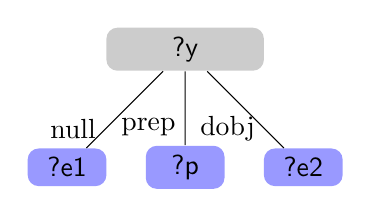
\begin{tikzpicture}
\node[fill = gray!40, shape = rectangle, rounded corners, minimum width = 2cm, font = \sffamily] (25) {?y}
child {node[fill = blue!40, shape = rectangle, rounded corners, minimum width = 1cm, font = \sffamily]  (26) {?e1}
}
child {node[fill = blue!40, shape = rectangle, rounded corners, minimum width = 1cm, font = \sffamily]  (27) {?p}
}
child {node[fill = blue!40, shape = rectangle, rounded corners, minimum width = 1cm, font = \sffamily]  (28) {?e2}
}
;
\begin{scope}[nodes = {draw = none}]
\path (26)     -- (25) node [near start, left]  {\text{null}};
\path (27)     -- (25) node [near start, left]  {\text{prep}};
\path (28)     -- (25) node [near start, left]  {\text{dobj}};
\draw[densely dashed, rounded corners, thin];
\end{scope} 
\end{tikzpicture}
\caption{Visualisation for SPARQLPattern\_EN\_9}
\label{fig:SPARQLPatternEN9}
\end{figure}


\end{document}